\chapter{Quantifying MGXS Approximations}
\label{chap:mgxs-approx-error}

%%%%%%%%%%%%%%%%%%%%%%%%%%%%%%%%%%%%%%%%%%%%%%%%%%%%%%%%%%%%%%%%%%%%%%%%%%%%%%%%
\section{Introduction}
\label{sec:chap4-intro}

\begin{itemize}[noitemsep]
  \item quantify \ac{MGXS} different approximation errors
  \item leave intra-pin spatial self-shielding error for later section
  \item need to discuss difference between iso-in-lab and regular scattering
\end{itemize}


%%%%%%%%%%%%%%%%%%%%%%%%%%%%%%%%%%%%%%%%%%%%%%%%%%%%%%%%%%%%%%%%%%%%%%%%%%%%%%%%
\section{Case Studies}
\label{sec:chap4-case-studies}

\begin{itemize}[noitemsep]
  \item \ac{MOC} convergence studies with \ac{MC}-generated \ac{MGXS}
  \begin{itemize}[noitemsep]
    \item track discretization
    \begin{itemize}[noitemsep]
      \item \# azimuthal angles
      \item track spacing
    \end{itemize}
    \item spatial discretization
    \item \# energy groups  
  \end{itemize}
  \item compare to reference \ac{MC} solution:
  \begin{itemize}
    \item eigenvalue
	\item Define $\Delta\rho$
    \item fluxes
  \end{itemize}
\end{itemize}

%%%%%%%%%%%%%%%%%%%%%%%%%%%%
\subsection{Infinite Medium}
\label{subsec:chap4-inf-medium}

-need super column with/without iso-in-lab scattering

\begin{itemize}[noitemsep]
\item table of isotopics
\item 128 azim angles
\item 0.01 cm track spacing
\item 1E-7 convergence threshold
\item double precision
\item reference $k_{eff}$ is 1.15912 $\pm$ 0.00009
\end{itemize}

\begin{table}[h!]
  \centering
  \caption{Angular-dependent $k_{eff}$ bias for an infinite medium.}
  \label{table:chap2-inf-med-angle}
  \vspace{14pt}
  \begin{tabular}{c S[table-format=2.1] S[table-format=2.1] S[table-format=2.1] c S[table-format=2.1] S[table-format=2.1] S[table-format=2.1]} 
  \toprule
  & \multicolumn{7}{c}{\boldmath $\Delta\rho$ {\bf [pcm]}} \\
  \midrule
  \multicolumn{1}{c}{\bf \# Angles} &
  \multicolumn{1}{c}{\bf 0.1 cm} & 
  \multicolumn{1}{c}{\bf 0.01 cm} & 
  \multicolumn{1}{c}{\bf 0.001 cm} &
  \multicolumn{1}{c}{} &
  \multicolumn{1}{c}{\bf 0.1 cm} & 
  \multicolumn{1}{c}{\bf 0.01 cm} & 
  \multicolumn{1}{c}{\bf 0.001 cm} \\
  \midrule
  & \multicolumn{3}{c}{\bf Anisotropic} &
  \multicolumn{1}{c}{} &
  \multicolumn{3}{c}{\bf Isotropic in Lab} \\
  \cline{2-4} \cline{6-8}
4 & 1.3 & 1.3 & 1.3 & & -0.1 & -0.1 & -0.1 \\
8 & 1.3 & 1.3 & 1.3 & & -0.1 & -0.1 & -0.1 \\
16 & 1.3 & 1.3 & 1.3 & & -0.1 & -0.1 & -0.1 \\
32 & 1.3 & 1.3 & 1.3 & & -0.1 & -0.1 & -0.1 \\
64 & 1.3 & 1.3 & 1.3 & & -0.1 & -0.1 & -0.1 \\
128 & 1.3 & 1.3 & 1.3 & & -0.1 & -0.1 & -0.1 \\
  \bottomrule
\end{tabular}
\end{table}

\begin{table}[h!]
  \centering
  \caption{Energy-dependent $k_{eff}$ bias for an infinite medium.}
  \label{table:chap2-inf-med-energy} 
  \vspace{14pt}
  \begin{tabular}{c S[table-format=2.1] S[table-format=2.1]}
  \toprule
  \multicolumn{1}{c}{\textbf{\# Groups}} &
  \multicolumn{2}{c}{\boldmath $\Delta\rho$ {\bf [pcm]}} \\
  \midrule
  & \multicolumn{1}{c}{\bf Anisotropic} &
  \multicolumn{1}{c}{\bf Isotropic in Lab} \\
  \midrule
1 & -11.1 & -10.5 \\
2 & -9.5 & -7.1 \\
4 & -0.1 & -0.5 \\
8 & 0.3 & -0.0 \\
16 & -0.2 & 0.5 \\
25 & 1.8 & 0.1 \\
40 & 1.6 & 0.1 \\
70 & 1.3 & -0.1 \\
  \bottomrule
\end{tabular}
\end{table}


%%%%%%%%%%%%%%%%%%%%
\subsection{1D Slab}
\label{subsec:chap4-slab}

\begin{itemize}[noitemsep]
  \item 1D slab equivalent to a representative \ac{PWR} fuel pin
  \item fuel, clad and moderator
  \item table of isotopics
  \item 128 azim angles
  \item 0.01 cm track spacing
  \item 1E-7 convergence threshold
  \item double precision
  \item use updated Falcon results
  \item reference $k_{eff}$ is 0.96304 $\pm$ 0.00009
\end{itemize}

-may need to use transport xs\\

\begin{table}[h!]
  \centering
  \caption{Angular-dependent $k_{eff}$ bias for a 1D slab.}
  \label{table:chap2-slab-angle}
  \vspace{14pt}
  \begin{tabular}{c S[table-format=4.1] S[table-format=4.1] S[table-format=2.1] c S[table-format=4.1] S[table-format=4.1] S[table-format=2.1]} 
  \toprule
  & \multicolumn{7}{c}{\boldmath $\Delta\rho$ {\bf [pcm]}} \\
  \midrule
  \multicolumn{1}{c}{\bf \# Angles} &
  \multicolumn{1}{c}{\bf 0.1 cm} & 
  \multicolumn{1}{c}{\bf 0.01 cm} & 
  \multicolumn{1}{c}{\bf 0.001 cm} &
  \multicolumn{1}{c}{} &
  \multicolumn{1}{c}{\bf 0.1 cm} & 
  \multicolumn{1}{c}{\bf 0.01 cm} & 
  \multicolumn{1}{c}{\bf 0.001 cm} \\
  \midrule
  & \multicolumn{3}{c}{\bf Anisotropic} &
  \multicolumn{1}{c}{} &
  \multicolumn{3}{c}{\bf Isotropic in Lab} \\
  \cline{2-4} \cline{6-8}
4 & -0.1 & -0.1 & -0.1 & & & & \\
8 & -0.1 & -0.1 & -0.1 & & & &  \\
16 & -0.1 & -0.1 & -0.1 & & & &  \\
32 & -0.1 & -0.1 & -0.1 & & & &  \\
64 & -0.1 & -0.1 & -0.1 & & & &  \\
128 & -0.1 & -0.1 & -0.1 & & & &  \\
  \bottomrule
\end{tabular}
\end{table}

\begin{table}[h!]
  \centering
  \caption{Energy-dependent $k_{eff}$ bias for a 1D slab.}
  \label{table:chap2-slab-energy} 
  \vspace{14pt}
  \begin{tabular}{c S[table-format=4.1] S[table-format=4.1] S[table-format=4.1] S[table-format=4.1] S[table-format=4.1]}
  \toprule
  & \multicolumn{5}{c}{\boldmath $\Delta\rho$ {\bf [pcm]}} \\
  \midrule  
  \multicolumn{1}{c}{\textbf{\# Groups}} &
  \multicolumn{1}{c}{\bf 1$\times$} &
  \multicolumn{1}{c}{\bf 2$\times$} &
  \multicolumn{1}{c}{\bf 4$\times$} &
%  \multicolumn{1}{c}{\bf 8$\times$} &
  \multicolumn{1}{c}{\bf 16$\times$} &
  \multicolumn{1}{c}{\bf 32$\times$} \\
  \midrule
  & \multicolumn{5}{c}{\bf Anisotropic} \\
  \cline{2-6}
1 &  &  &  &  & \\
  & \multicolumn{5}{c}{\bf Isotropic in Lab} \\
  \cline{2-6}
1 &  &  &  &  & \\
  \bottomrule
\end{tabular}
\end{table}

\begin{table}[h!]
  \centering
  \caption{Spatial-dependent $k_{eff}$ bias for a 1D slab.}
  \label{table:chap2-slab-space} 
  \vspace{14pt}
  \begin{tabular}{c S[table-format=4.1] S[table-format=4.1] S[table-format=4.1] S[table-format=4.1] S[table-format=4.1]}
  \toprule
  & \multicolumn{5}{c}{\boldmath $\Delta\rho$ {\bf [pcm]}} \\
  \midrule  
  \multicolumn{1}{c}{\textbf{\# Groups}} &
  \multicolumn{1}{c}{\bf 1$\times$} &
  \multicolumn{1}{c}{\bf 2$\times$} &
  \multicolumn{1}{c}{\bf 4$\times$} &
%  \multicolumn{1}{c}{\bf 8$\times$} &
  \multicolumn{1}{c}{\bf 16$\times$} &
  \multicolumn{1}{c}{\bf 32$\times$} \\
  \midrule
  & \multicolumn{5}{c}{\bf Anisotropic} \\
  \cline{2-6}
1 & 4253 & 4750 & 5094 & 5263 & 5271 \\
2 & 8797 & 4796 & 404 & -2817 & -3062 \\
4 & 8983 & 4754 & -65 & -3610 & -3876 \\
8 & 10080 & 5329 & -201 & -4491 & -4826 \\
16 & 10184 & 5422 & -92 & -4401 & -4742 \\
25 & 10262 & 5519 & -63 & -4436 & -4780 \\
40 & 10366 & 5611 & 4 & -4411 & -4758 \\
70 & 10387 & 5633 & 19 & -4406 & -4756 \\
  & \multicolumn{5}{c}{\bf Isotropic in Lab} \\
  \cline{2-6}
1 & 4654 & 5303 & 5731 & 5972 & 6011 \\
2 & 13926 & 9470 & 4647 & 1130 & 883 \\
4 & 13752 & 9266 & 4241 & 540 & 266 \\
8 & 15103 & 10190 & 4546 & 169 & -165 \\
16 & 15194 & 10282 & 4658 & 269 & -68 \\
25 & 15089 & 10319 & 4723 & 322 & -17 \\
40 & 15165 & 10395 & 4783 & 351 & 9 \\
70 & 15177 & 10416 & 4803 & 370 & 29 \\
  \bottomrule
\end{tabular}
\end{table}


%%%%%%%%%%%%%%%%%%%%%%%%%%%%%
\subsection{2D Fuel Pin Cell}
\label{subsec:chap4-pin}

\begin{itemize}[noitemsep]
  \item 2D fuel pin from \ac{BEAVRS}
  \item fuel, clad, gap and moderator
\end{itemize}

\begin{table}[h!]
  \centering
  \caption{Angular-dependent $k_{eff}$ bias for a 2D fuel pin.}
  \label{table:chap2-pin-angle}
  \vspace{14pt}
  \begin{tabular}{c S[table-format=2.1] S[table-format=2.1] S[table-format=2.1] c S[table-format=2.1] S[table-format=2.1] S[table-format=2.1]} 
  \toprule
  & \multicolumn{7}{c}{\boldmath $\Delta\rho$ {\bf [pcm]}} \\
  \midrule
  \multicolumn{1}{c}{\bf \# Angles} &
  \multicolumn{1}{c}{\bf 0.1 cm} & 
  \multicolumn{1}{c}{\bf 0.01 cm} & 
  \multicolumn{1}{c}{\bf 0.001 cm} &
  \multicolumn{1}{c}{} &
  \multicolumn{1}{c}{\bf 0.1 cm} & 
  \multicolumn{1}{c}{\bf 0.01 cm} & 
  \multicolumn{1}{c}{\bf 0.001 cm} \\
  \midrule
  & \multicolumn{3}{c}{\bf Anisotropic} &
  \multicolumn{1}{c}{} &
  \multicolumn{3}{c}{\bf Isotropic in Lab} \\
  \cline{2-4} \cline{6-8}
4 & -0.1 & -0.1 & -0.1 & & & & \\
8 & -0.1 & -0.1 & -0.1 & & & &  \\
16 & -0.1 & -0.1 & -0.1 & & & &  \\
32 & -0.1 & -0.1 & -0.1 & & & &  \\
64 & -0.1 & -0.1 & -0.1 & & & &  \\
128 & -0.1 & -0.1 & -0.1 & & & &  \\
  \bottomrule
\end{tabular}
\end{table}

\begin{table}[h!]
  \centering
  \caption{Energy-dependent $k_{eff}$ bias for a 2D fuel pin.}
  \label{table:chap2-pin-energy} 
  \vspace{14pt}
  \begin{tabular}{c S[table-format=2.1] S[table-format=2.1] S[table-format=2.1] S[table-format=2.1] S[table-format=2.1] S[table-format=2.1]}
  \toprule
  & \multicolumn{6}{c}{\boldmath $\Delta\rho$ {\bf [pcm]}} \\
  \midrule  
  \multicolumn{1}{c}{\textbf{\# Groups}} &
  \multicolumn{1}{c}{\bf 1$\times$} &
  \multicolumn{1}{c}{\bf 2$\times$} &
  \multicolumn{1}{c}{\bf 4$\times$} &
  \multicolumn{1}{c}{\bf 8$\times$} &
  \multicolumn{1}{c}{\bf 16$\times$} &
  \multicolumn{1}{c}{\bf 32$\times$} \\
  \midrule
  & \multicolumn{6}{c}{\bf Anisotropic} \\
  \cline{2-7}
  1 & & & & & & \\
  2 & & & & & & \\
  4 & & & & & & \\
  8 & & & & & & \\
  16 & & & & & & \\
  25 & & & & & & \\
  40 & & & & & & \\
  70 & & & & & & \\
  & \multicolumn{6}{c}{\bf Isotropic in Lab} \\
  \cline{2-7}
  1 & & & & & & \\
  2 & & & & & & \\
  4 & & & & & & \\
  8 & & & & & & \\
  16 & & & & & & \\
  25 & & & & & & \\
  40 & & & & & & \\
  70 & & & & & & \\  
  \bottomrule
\end{tabular}
\end{table}

\begin{table}[h!]
  \centering
  \caption{Spatial-dependent $k_{eff}$ bias for a 2D fuel pin.}
  \label{table:chap2-pin-space} 
  \vspace{14pt}
  \begin{tabular}{c S[table-format=2.1] S[table-format=2.1] S[table-format=2.1] S[table-format=2.1] S[table-format=2.1] S[table-format=2.1]}
  \toprule
  & \multicolumn{6}{c}{\boldmath $\Delta\rho$ {\bf [pcm]}} \\
  \midrule  
  \multicolumn{1}{c}{\textbf{\# Groups}} &
  \multicolumn{1}{c}{\bf 1$\times$} &
  \multicolumn{1}{c}{\bf 2$\times$} &
  \multicolumn{1}{c}{\bf 4$\times$} &
  \multicolumn{1}{c}{\bf 8$\times$} &
  \multicolumn{1}{c}{\bf 16$\times$} &
  \multicolumn{1}{c}{\bf 32$\times$} \\
  \midrule
  & \multicolumn{6}{c}{\bf Anisotropic} \\
  \cline{2-7}
  1 & & & & & & \\
  2 & & & & & & \\
  4 & & & & & & \\
  8 & & & & & & \\
  16 & & & & & & \\
  25 & & & & & & \\
  40 & & & & & & \\
  70 & & & & & & \\
  & \multicolumn{6}{c}{\bf Isotropic in Lab} \\
  \cline{2-7}
  1 & & & & & & \\
  2 & & & & & & \\
  4 & & & & & & \\
  8 & & & & & & \\
  16 & & & & & & \\
  25 & & & & & & \\
  40 & & & & & & \\
  70 & & & & & & \\  
  \bottomrule
\end{tabular}
\end{table}

-make plots without SPH\\

\begin{figure}[h!]
  \centering
  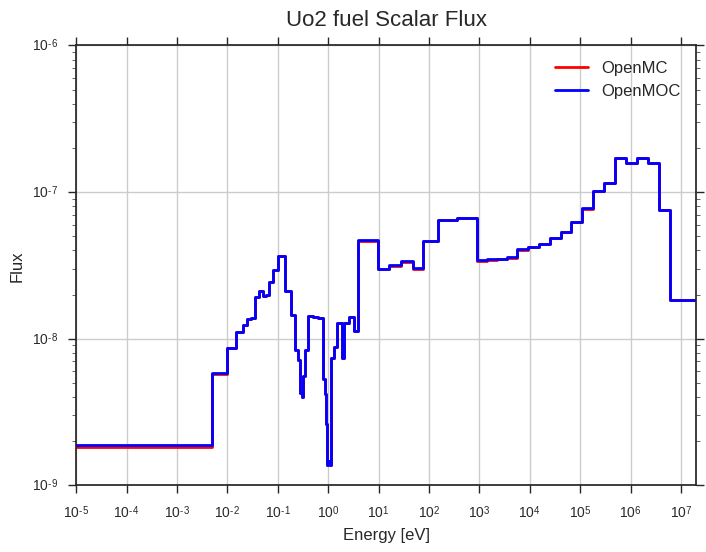
\includegraphics[width=0.9\linewidth]{figures/biases/pin-cell/flux-uo2-fuel}
  \caption{}
\label{fig:chap2-pin-flux}
\end{figure}

\begin{figure}[h!]
  \centering
  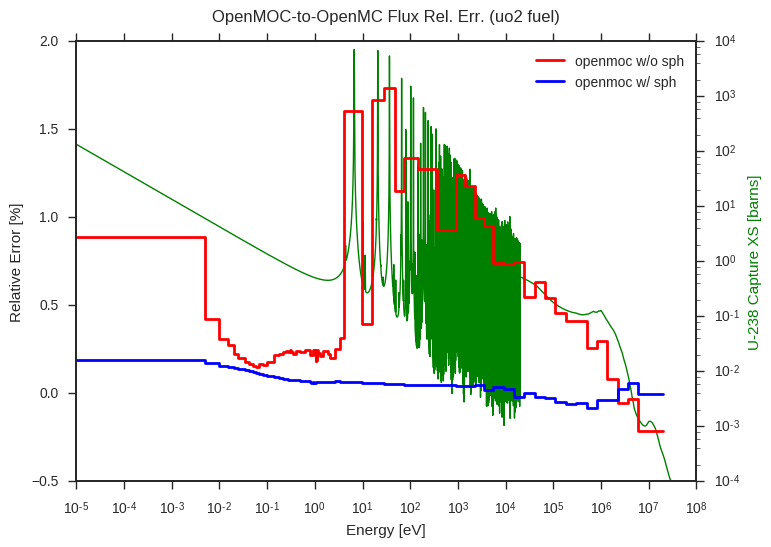
\includegraphics[width=0.9\linewidth]{figures/biases/pin-cell/rel-err-uo2-fuel}
  \caption{}
\label{fig:chap2-pin-flux}
\end{figure}


%%%%%%%%%%%%%%%%%%%%%%%%%%%%%%%%%%%%%%%%%%%
\subsection{2D Fuel Assembly}

\begin{table}[h!]
  \centering
  \caption{Angular-dependent $k_{eff}$ bias for a 2D fuel assembly.}
  \label{table:chap2-lattice-angle}
  \vspace{14pt}
  \begin{tabular}{c S[table-format=2.1] S[table-format=2.1] S[table-format=2.1] c S[table-format=2.1] S[table-format=2.1] S[table-format=2.1]} 
  \toprule
  & \multicolumn{7}{c}{\boldmath $\Delta\rho$ {\bf [pcm]}} \\
  \midrule
  \multicolumn{1}{c}{\bf \# Angles} &
  \multicolumn{1}{c}{\bf 0.1 cm} & 
  \multicolumn{1}{c}{\bf 0.01 cm} & 
  \multicolumn{1}{c}{\bf 0.001 cm} &
  \multicolumn{1}{c}{} &
  \multicolumn{1}{c}{\bf 0.1 cm} & 
  \multicolumn{1}{c}{\bf 0.01 cm} & 
  \multicolumn{1}{c}{\bf 0.001 cm} \\
  \midrule
  & \multicolumn{3}{c}{\bf Anisotropic} &
  \multicolumn{1}{c}{} &
  \multicolumn{3}{c}{\bf Isotropic in Lab} \\
  \cline{2-4} \cline{6-8}
4 & -0.1 & -0.1 & -0.1 & & & & \\
8 & -0.1 & -0.1 & -0.1 & & & &  \\
16 & -0.1 & -0.1 & -0.1 & & & &  \\
32 & -0.1 & -0.1 & -0.1 & & & &  \\
64 & -0.1 & -0.1 & -0.1 & & & &  \\
128 & -0.1 & -0.1 & -0.1 & & & &  \\
  \bottomrule
\end{tabular}
\end{table}

\begin{table}[h!]
  \centering
  \caption{Energy-dependent $k_{eff}$ bias for a 2D fuel assembly.}
  \label{table:chap2-lattice-energy} 
  \vspace{14pt}
  \begin{tabular}{c S[table-format=2.1] S[table-format=2.1] S[table-format=2.1] S[table-format=2.1] S[table-format=2.1] S[table-format=2.1]}
  \toprule
  & \multicolumn{6}{c}{\boldmath $\Delta\rho$ {\bf [pcm]}} \\
  \midrule  
  \multicolumn{1}{c}{\textbf{\# Groups}} &
  \multicolumn{1}{c}{\bf 1$\times$} &
  \multicolumn{1}{c}{\bf 2$\times$} &
  \multicolumn{1}{c}{\bf 4$\times$} &
  \multicolumn{1}{c}{\bf 8$\times$} &
  \multicolumn{1}{c}{\bf 16$\times$} &
  \multicolumn{1}{c}{\bf 32$\times$} \\
  \midrule
  & \multicolumn{6}{c}{\bf Anisotropic} \\
  \cline{2-7}
  1 & & & & & & \\
  2 & & & & & & \\
  4 & & & & & & \\
  8 & & & & & & \\
  16 & & & & & & \\
  25 & & & & & & \\
  40 & & & & & & \\
  70 & & & & & & \\
  & \multicolumn{6}{c}{\bf Isotropic in Lab} \\
  \cline{2-7}
  1 & & & & & & \\
  2 & & & & & & \\
  4 & & & & & & \\
  8 & & & & & & \\
  16 & & & & & & \\
  25 & & & & & & \\
  40 & & & & & & \\
  70 & & & & & & \\  
  \bottomrule
\end{tabular}
\end{table}
